\documentclass{oci}
\usepackage[utf8]{inputenc}
\usepackage{lipsum}
\usepackage{tikz}

\title{Ejemplo}

\begin{document}
\begin{problemDescription}
  En una tarde aburrida en su casa Alicia inventó un juego muy particular.
  Para poder jugarlo solo se necesita un lápiz y el calendario de un mes de 30 días.
  Comenzando en un día $x$ del mes, el juego consiste en aplicar una serie de reglas para
  moverse entre los días del mes tachando cada día visitado.
  El juego termina al visitar un día que ya había sido tachado o no es posible aplicar
  una regla.
  Las reglas específicas se detallan más adelante.

  Los días del mes se numeran de 1 a 30.
  Dependiendo del mes, el primer día puede caer en distintos días de la semana y esto cambiará
  el desarrollo del juego.
  La siguiente imagen muestra el calendario de un mes donde el primer día cae un viernes.
  \begin{center}
    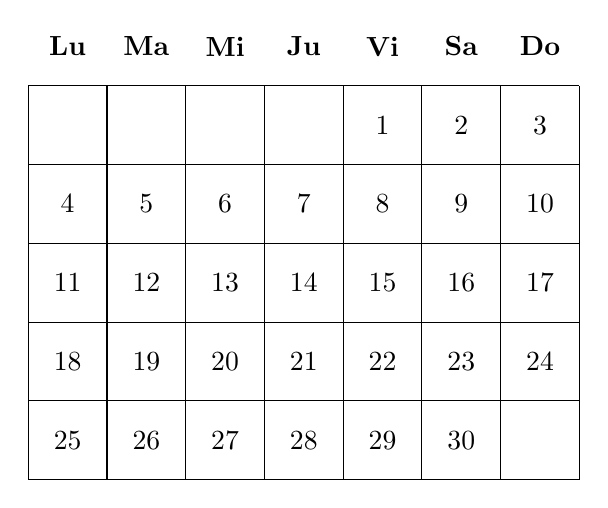
\begin{tikzpicture}
      \draw (0, 0) grid (7, 5);
      \def\weeks{5}
      \def\start{4}
      \foreach \d [count=\x from 0] in {Lu, Ma, Mi, Ju, Vi, Sa, Do}{
        \node at (\x + 0.5, \weeks + 0.5) {\textbf{\d}};
      };
      \foreach \i in {0, ..., 29}{
        \pgfmathtruncatemacro{\x}{Mod(\start + \i, 7)}
        \pgfmathtruncatemacro{\y}{(\start + \i) / 7}
        \pgfmathtruncatemacro{\d}{\i + 1}
        \node[fill=white] at (\x + 0.5, \weeks - \y - 0.5) {\d};
      }
    \end{tikzpicture}
  \end{center}

  A continuación se describe en detalle las reglas del juego.
  La regla que hay que aplicar depende del día de la semana del día actual.

  \begin{description}
    \item[Lunes] Avanzar de uno en uno hasta encontrar un día no tachado y moverse a este día.
    Si no queda ningún día sin tachar la regla no puede aplicarse y el juego termina en el día actual.
    \item[Martes] Moverse al día correspondiente al reflejo del día actual con respecto al centro
    del mes, es decir, si el día actual es $i$ moverse al día $30 - i + 1$.
    \item[Miércoles] Si el día actual es par, moverse al día siguiente. En caso contrario, moverse al día anterior.
    \item[Jueves] Moverse 10 días adelante.
    Si el día cae fuera del mes dar la vuelta al mes.
    Por ejemplo si el día actual es 28 moverse al día 8.
    \item[Viernes] Si el día actual $i$ es par, moverse al día $i/2$. En caso contrario, moverse al día $3\times i + 1$.
    Si el día cae fuera del mes dar vueltas al mes cuantas veces sea necesario.
    \item[Sábado] Si el día actual es $i$ moverse al día $2\times i$ dando las vueltas al mes cuantas veces sea necesario.
    \item[Domingo] Avanzar de dos en dos hasta encontrar un día no tachado.
    Si no queda ningún día sin tachar la regla no puede aplicarse y el juego termina en el día actual.
  \end{description}
\end{problemDescription}

\begin{inputDescription}
  La entrada contiene una línea con dos enteros $d$ ($0 \leq d \leq 6$) y $x$ ($1 \leq x \leq 30$).
  El entero $d$ corresponde al día de la semana en que cae el primer día del mes.
  Si $d$ es $0$ el mes comienza un lunes, si $d$ es $1$ el mes comienza un martes y así hasta el domingo.
  El entero $x$ indica el día del mes en que comienza el juego.
\end{inputDescription}

\begin{outputDescription}
  La salida debe contener un único entero indicando el día del mes en el que termina el juego.
\end{outputDescription}

\begin{scoreDescription}
  Este enunciado no contiene subtareas, se entregará puntaje proporcional a la cantidad de casos
  de prueba correctos siendo 100 el puntaje máximo.
  % \subtask{40}
  % Se probarán varios casos donde $d = 0$, es decir, el mes siempre comienza un lunes.
  % \subtask{60}
  % Se probarán varios casos sin restricciones adicionales.
\end{scoreDescription}

\begin{sampleDescription}
\sampleIO{sample-1}
\sampleIO{sample-2}
\end{sampleDescription}

\end{document}
